%% Los cap'itulos inician con \chapter{T'itulo}, estos aparecen numerados y
%% se incluyen en el 'indice general.
%%
%% Recuerda que aqu'i ya puedes escribir acentos como: 'a, 'e, 'i, etc.
%% La letra n con tilde es: 'n.

\chapter{Modelo $\mathcal{G}^0$}
\label{modeloG0}

Las imágenes adquiridas por radares de apertura sintética SAR han encontrado muchas aplicaciones debido a sus ventajas respecto de las imágenes que provienen de sensores ópticos. La independencia de las condiciones climáticas y de la iluminación junto con la capacidad de penetrar la nubes, las copas de los árboles e incluso el suelo, han contribuido para que este tipo de imágenes resulten cada vez más populares.

Sin embargo, las imágenes SAR tienen la desventaja de ser difíciles de interpretar y procesar debido a la presencia del ruido speckle. Como hemos visto en capítulos anteriores, este ruido es inherente al proceso de captura de la imagen y se hace presente debido a la superposición coherente de las ondas reflejadas por muchos dispersores. Esto causa una variación en la intensidad pixel a pixel que se manifiesta en la imagen como un patrón granular. 

Debido a la aleatoriedad y a la fuerte dispersión que puede tener la señal retrodispersada, es necesario contar con modelos estadísticos que contribuyan a una mejor extracción de información a través del desarrollo de filtros, detección de bordes, clasificación de áreas entre otras metodologías. 

El modelo multiplicativo es muy apropiado para explicar las características estadísticas de la imagen de un objeto cuando es iluminado por radiación coherente, como lo son las imágenes SAR.
Este modelo considera que el valor observado en cada celda de la imagen es una variable aleatoria $Z$ que resulta del producto de dos variables aleatorias independientes: una correspondiente a la retrodispersión $X$ (que es lo que observaríamos sin la presencia del ruido speckle) y la otra correspondiente al ruido speckle $Y$ (que es inherente a todo sistema de captura de imágenes con iluminación coherente).

%El modelo Rayleigh ajusta razonablemente bien para áreas homogéneas pero a veces falla en el caso de áreas heterogéneas. Lee y Pottier \citet{Lee2009} explican la naturaleza multiplicativa del ruido speckle realizando un scatter plot del desvío estandard respecto de la media muestral en muchas zonas homogéneas en una imagen SAR. Si se supone un backscatter constante $\mathrm{C}$ en zonas homogéneas, el retorno queda modelado por $\mathrm{Z}=\mathrm{C} \cdot \mathrm{Y}$. Entonces, calculando la esperanza y el desvío de $\mathrm{Z}$ se obtiene
%\begin{align}
%\mathrm{E(Z)}&=C \, \mathrm{E(Y)}\label{esperanza}\\
%\mathrm{SD(Z)}&=C \cdot \mathrm{SD(Y)}\label{desvio}
%\end{align} 
%Despejando $C$ de~\eqref{esperanza} y reemplanzando en~\eqref{desvio} se obtiene que
%\begin{align}
%\mathrm{SD(Z)}&= \mathrm{\dfrac{SD(Y)}{E(Y)}} \, \mathrm{E(Z)}\label{desvio}
%\end{align} 
%En la figura~\ref{ModeloMultiplicativo} tomada de Lee y Pottier \citet{Lee2009} se muestra un scatter plot basado en datos tomados por el radar SIR-B (Spaceborne Imaging Radar), un sensor SAR que opera en banda $\mathrm{C}$ y $\mathrm{X}$. Estos datos están en formato amplitud.
%\begin{figure}[hbt]
%	\centering    
%	\includegraphics[scale=0.5]{../../Figures/Tesis/Capitulo4/ModeloMultiplicativo.png}
%	\caption{\label{ModeloMultiplicativo}Modelo Multiplicativo.} %Fuente Canada Centre for Remote Sensing \citet{ccrs2001}.}
%\end{figure} 
%En esta figura se puede observar que la naturaleza multiplicativa del ruido speckle se manifiesta en la recta que pasa por el origen producto del ajuste lineal que se realizó al conjunto de datos. De acuerdo a Lee y Pottier \citet{Lee2009} los valores de las pendiendes para $1$-look y $4$-look son $0.54$ y $0.26$ respectivamente, que son razonablemente cercanos a los valores teóricos $0.5227$ y $0.261$ respectivamente.

Se han utilizado algunos distribuciones estadísticas para modelar los datos SAR, \citet{Lee2009} presentan la distribución Lognormal, la Weibull y la distribución $\mathcal{K}$. 

\citet{Frery97} indican que un modelo común para datos que provienen de zonas homogéneas y con mucha presencia de ruido speckle son la distribución exponencial y la Rayleigh. En cambio las distribuciones $\mathcal{K}$ que presentan \citet{Jakeman87} han sido muy utilizada en datos SAR especialmente cuando los datos provienen de áreas texturadas. 

 \citet{Frery97} y \citet{Frery99} presentan la familia de distribuciones $\mathcal{G}$ para datos dados tanto en formato amplitud como en intensidad, generando la familia de distribuciones $\mathcal{G}_A$ y $\mathcal{G}_I$ respectivamente. Es un modelo más general porque distribuciones clásicas, como $\mathcal{K}$, son casos particulares de esta nueva familia de distribuciones.

Como caso particular de esta clase de distribuciones está la familia $\mathcal{G}^0$ que tiene tantos parámetros como la distribución $\mathcal{K}$ y es capaz de modelar zonas extremadamente rugosas, como las zonas urbanas, mejor que esta útlima distribución como lo indica \citet{Mejail99}. 

La familia de distribuciones $\mathcal{G}^0$ está indexadas por tres parámetros: $\alpha$ que está relacionado con la textura del terreno, el parámetro $\gamma$ considerado un parámetro de escala e informa sobre el brillo de la imagen y el parámetro $L$ que es el número de looks. Este último parámetro da información sobre la relación señal-ruido de la imagen, cuanto mayor es el número de looks menor presencia de ruido speckle se encuentra en la imagen, a expensas de una pérdida en la resolución. Esta familia también modela datos en formato amplitud como en intensidad generando la familia de distribuciones $\mathcal{G}_A^0$ como lo indican \citet{Frery97}, y la familia de distribuciones $\mathcal{G}_I^0$ de acuerdo a \citet{Frery97,Frery99} respectivamente. En esta tesis se trabajará con datos dados en formato intensidad.

En este capítulo se presenta el modelo multiplicativo junto con la distribución $\mathcal{G}_I^0$ y la relación con otras distribuciones. Asimismo se presentan resultados teóricos producto de esta tesis, donde se muestra la capacidad que tiene esta distribución de generar valores atípicos, y resultados de convergencia uniforme de la distribución $\mathcal{G}_I^0$ cuando el parámetro de textura $\alpha \longrightarrow -1$ y cuando $\alpha \longrightarrow -\infty$.

%\begin{figure}[hbt]
%	\centering    
%	\includegraphics[scale=0.5]{../../Figures/Tesis/Capitulo4/RelacionDistribuciones.png}
%	\caption{\label{RelacionDistribuciones}Relación entre los modelos estadísticos más usados.} %Fuente Canada Centre for Remote Sensing~\cite{ccrs2001}.}
%\end{figure} 

\section{Modelo Multiplicativo}
\label{ModeloMultiplicativo}

Una aproximación para comprender la distribución de los datos SAR es proponer modelos que ajusten razonablemente bien a ellos. Algunas distribuciones conocidas como la Exponencial, Gamma, Lognormal, Rayleig, Weibull entre otras, fueron propuestas como "modelos empíricos"  para describir a los datos SAR. En \citet{FreryLibro2019}, \citet{oliverquegan98}, \citet{Yanasse93} y \citet{Lee2009} se pueden ver referencias a estos modelos. La pertinencia de estas distribuciones depende del formato de los datos (amplitud, intensidad, complejo, etc.), el número de looks y el grado de homogeneidad de la zona bajo estudio.

%
%Muchas distribuciones univariadas han sido propuestas para modelar el retorno $Z$ conocidas como "modelos empíricos". Dentro de estas distribuciones se encuentran la distribución Exponential, Gamma, Lognormal, Weibull entre otras \citet{FreryLibro2019,Gao2010}. La pertinencia de estas distribuciones depende del formato de los datos (amplitud, intensidad, complejo, etc.), el número de looks y el grado de homogeneidad de la zona bajo estudio.

%Una aproximación para comprender la distribución de los datos SAR es proponer modelos que ajusten razonablemente bien a estos datos. Alguna distribuciones conocidas como la Lognormal \citet{oliverquegan98}, Rayleig, Weibull \citet{Lee2009} fueron propuestas como "modelos empíricos" para describir este tipo de datos. Todas estas distribuciones fueron estudiadas en \citet{Yanasse93,Lee2009} entre otros autores.

 \citet{Lee2009} explican la naturaleza multiplicativa del ruido speckle utilizando el modelo Rayleigh para $1$-look con datos en formato amplitud en zonas homogéneas. Ellos realizaron un scatter plot del desvío standard muestral respecto de la media muestral en muchas zonas homogéneas en una imagen SAR. Para el caso de $n$ muestras provenientes de una imagen de $1$-look utilizan en modelo Rayleigh. En el caso de muestras de $4$-looks modelan con la distribución $\chi$ con $2n$ grados de libertad.

Si se supone una retrodispersión constante $C$ en zonas homogéneas, el retorno queda modelado por $Z=C \cdot Y$ bajo el modelo multiplicativo. Entonces, calculando la esperanza y el desvío de $Z$ se obtiene

\begin{align}
E(Z)&=C \, E(Y)\label{esperanza}\\
SD(Z)&=C \cdot SD(Y)\label{desvio}
\end{align} 

%\begin{align}
%\mathrm{E(Z)}&=C \, \mathrm{E(Y)}\label{esperanza}\\
%\mathrm{SD(Z)}&=C \cdot \mathrm{SD(Y)}\label{desvio}
%\end{align} 
Despejando $C$ de~\eqref{esperanza} y reemplanzando en~\eqref{desvio} se obtiene que
\begin{align}
SD(Z)&= \dfrac{SD(Y)}{E(Y)} \, E(Z)
\end{align} 
En la figura~\ref{ModeloMultiplicativo} tomada de \citet{Lee2009} se muestra el \textit{scatter plot} basado en datos tomados por el radar SIR-B (Spaceborne Imaging Radar), un sensor SAR que opera en banda $C$ y $X$. Se tomaron $16$ y $25$ muestras de zonas homogéneas para el caso de $1$-look y $4$-looks respectivamente. En cada muestra se calculó $\overline{}$ la media muestral y $SD$ el desvío muestral y se grafica $SD$ vs. $\overline{Z}.$

\begin{figure}
\centering
\begin{overpic}
	[scale=0.5]{../../Figures/Tesis/Capitulo4/ModeloMultiplicativo2.pdf}
	\put(13,153){\rotatebox[origin=c]{90}{SD}}
	\put(150,15){$\bar{Z}$}
\end{overpic}
\caption{\label{Modelo Multiplicativo}Modelo Multiplicativo, fuente Lee et.al \citet{Lee2009}.}
\end{figure}

La naturaleza multiplicativa del ruido speckle se manifiesta en la recta que pasa por el origen producto del ajuste lineal que se realizó al conjunto de datos. De acuerdo a \citet{Lee2009} los valores de las pendiendes para $1$-look y $4$-look son $0.54$ y $0.26$ respectivamente, que son razonablemente cercanos a los valores teóricos $0.5227$ y $0.261$ respectivamente.

Por este motivo en este tesis se utilizará el modelo multiplicativo para modelar datos SAR. Este enfoque se basa en la física de la formación de la imagen donde toma en cuenta la iluminación coherente propia de este tipo de sensores y propone aprovechar la naturaleza multiplica del ruido speckle.

El modelo multiplicativo considerado es el siguiente:
\begin{equation*}
Z=X \cdot Y  
\end{equation*}
donde $X$ e $Y$ corresponden a la retrodispersión e $Y$ corresponde al ruido speckle, respectivamente.

En esta tesis se consideran imágenes monopolarimétricas, una banda y una polarización en formato intensidad. Daremos modelos para el speckle, la retrodispersión y finalmente para el retorno bajo el modelo multiplicativo.


\section{Modelo para el Ruido Speckle}
\label{ModeloSpeckle}

De acuerdo a la ecuación~\eqref{RetornoComplejo} el retorno $S$ es un número complejo. Entonces $S=S_{\text{R}}+i \, S_{\text{Im}}$ donde $i$ es la unidad imaginaria, $S_{\text{R}}$ y $S_{\text{Im}}$ son la parte real e imaginaria de $S$ respectivamente. Entonces $Z=S_{\text{R}}^2+S_{\text{Im}}^2$ donde $Z$ es la intensidad del retorno. 

 \citet{FreryLibro2019} indican que, dadas las condiciones:
\begin{itemize}
	\item retrodispersores con tamaño menor que la longitud de onda,
	\item amplitudes $A_j$ de los dispersores elementales independientes y positivas,
	\item ningún retrodispersor dominante, 
	\item fases $\phi_i$ independientes e igualmente distribuidas con distribución uniforme en $[-\pi,\pi]$,
\end{itemize}   
se puede probar que $S_{\text{R}} \sim N(0,\sigma^2/2)$ y $S_{\text{Im}} \sim N(0,\sigma^2/2)$. Entonces
\begin{align}
\label{DistRetornoExp}
	Z \sim Exp(1/\sigma^2) \equiv \Gamma(1,1/\sigma^2),
\end{align}
donde $\sigma^2$ es la intensidad media del retorno.

Cabe señalar que en esta tesis se van a considerar las siguientes parametrizaciones para las distribuciones $Exp(\lambda)$ y $\Gamma(\alpha,\beta)$. Sean $T \sim Exp(\lambda)$ y $W \sim \Gamma(\alpha,\beta)$ entonces las funciones de densidad $f_{\text{T}}$ y $f_{\text{W}}$ están dadas por
\begin{align}
f_{\text{T}}(t)&=\lambda e^{-\lambda t}\label{DistExponencial}\\
f_{\text{w}}(t)&=\dfrac{\beta^{\alpha}}{\Gamma(\alpha)} t^{\alpha-1} e^{-\beta \, t}\label{DistGamma}
\end{align}
respectivamente.  

Entonces, si modelamos a $X$ como la intensidad media del retorno $\sigma^2$, el modelo para $Z$ para $1$-look será $Z=\sigma^2 \, Y$, donde $Y \sim \Gamma(1,1)$ es el modelo para el ruido speckle.
 
Como se vio en la sección~\ref{FormacionSpeckle} una técnica muy utilizada para disminuir el efecto del ruido speckle en la imagen SAR y, por lo tanto, mejorar la relación señal-ruido es el proceso multilook. Este proceso consiste en promediar $L$ vistas independientes de retornos de $1$-look. Entonces la intensidad del retorno final es el promedio de las intensidades de los retornos $Z_l$ de cada una de estas vistas. Es decir 
\begin{align}
Z=\dfrac{1}{L}\sum_{l=1}^L Z_l.
\end{align}

Entonces, por~\eqref{DistRetornoExp} y utilizando propiedades de la distribución $\Gamma(\alpha,\beta)$, $Z$  queda distribuido como $Z \sim \Gamma(L,L/\sigma^2)$. Entonces, si consideramos a la retrodispersión constante, el retorno $Z$ para el caso de $L$-looks queda modelado como
\begin{align}
Z=\sigma^2 \, Y \text{ con } Y \sim \Gamma(L,L).
\end{align}

La pregunta que nos podemos hacer es ¿tiene sentido considerar un retrodispersor constante? Y, obviamente, la respuesta es no. Dependiendo cómo se modele a $X$ surgen distintas familas de distribuciones para modelar el retorno.

Si $X \sim \Gamma(\alpha,\lambda)$ entonces $Z \sim \mathcal{K}(\alpha,\lambda,L)$, donde la función de densidad está dada por
\begin{align}
f_{\text{Z}}(z)&=\frac{2 z^{\frac{1}{2} (L+\alpha-2 )} (L \lambda )^{\frac{L+\alpha }{2}} K_{\alpha -L}\left(2 \sqrt{L x
		\lambda }\right)}{\Gamma (L) \Gamma (\alpha )}.
\end{align}
 Esta familia de distribuciones fueron propuestas por \citet{Jakeman87} y ha sido un modelo ampliamente utilizado, pero no modela en forma adecuada datos que provienen de zonas extremadamente heterogéneas como son las áreas urbanas como lo indicaron en \citet{Frery97}.

 \citet{Frery99} propusieron un nuevo modelo para la retrodispersión, dando origen a una nueva familia de distribuciones que modelan muy bien datos provenientes de zonas extremadamente heterogéneas mejor que la familia $\mathcal{K}$. Esta familia de distribuciones se llama $\mathcal{G}$ y fueron ampliamente aplicadas por  \citet{gambini2015} y \citet{Nascimento2009} en imágenes monopolarimétricas. \citet{Freitas2005} y \citet{Palacio2019} utilizaron esta familia de distribuciones en imágenes polarimétricas.

\section{Modelo para la Retrodispersión}
\label{ModeloBackscatter}

El grado de homogeneidad de un área de la imagen está modelado por la retrodispersión. Por este motivo es importante encontrar un modelo que sea lo más general posible, para que pueda explicar los diferentes grados de textura que tiene una imagen.

 \citet{Frery99} consideraron un modelo general para la retrodispersión que tiene como casos especiales modelos más simples que permiten explicar las diferentes texturas que puede tener un determinado área. En general, estas texturas se indican como: áreas homogéneas (pastura), heterogéneas (bosque) y extremadamente heterogéneas (áreas urbanas). Estos modelos simples tienen la ventaja de tener menos parámetros para estimar.

El modelo que proponen en \citet{Frery99} para la retrodispersión en el caso de datos de intensidad es una distribución Gaussiana Inversa Generalizada con parámetros $\alpha$, $\gamma$ y $\lambda$. En este caso decimos que  $X\sim N^{-1}(\alpha,\gamma,\lambda)$ cuya función de densidad viene dada por
\begin{align}
f_X(x) = \dfrac{\left(\frac{\lambda}{\gamma}\right)^{\frac{\alpha}{2}}}{2 \text{K}_{\alpha} (2 \sqrt{\lambda \gamma})} x^{\alpha-1} e^{-\frac{\gamma}{x}-\lambda x} \text{ para } x>0,
\label{GIG}
\end{align}
donde $\text{K}_{\alpha}$ indica la función de Bessel modificada de tercera especie y de orden $\alpha$. 

El espacio paramétrico está dado por
\begin{align}
\begin{cases}
\label{EspacioParametros}
	\gamma>0,      \,  \lambda \geq 0,  & \text{ si } \alpha < 0\\
	\gamma>0,      \,  \lambda >0,      & \text{ si } \alpha=0\\
	\gamma \geq 0, \,  \lambda >0,      & \text{ si } \alpha>0.
\end{cases}
\end{align}

Este modelo general presenta algunas ventajas porque tiene como casos particulares a algunas distribuciones que son muy utilizadas para modelar el retorno para datos en formato intensidad. Estos casos son:

\begin{itemize}
	\item Una constante $C$ que se utiliza para modelar áreas homogéneas dando lugar a un retorno que es puro speckle. Este caso lo vimos anteriormente y da lugar a un retorno modelado con una distribución Gamma.
	\item La distribución Gamma, dando lugar a la familia de distribuciones $\mathcal{K}$. 
	\item La distribución Gamma Inversa ($\Gamma^{-1}$) dando lugar a la familia de distribuciones $\mathcal{G}_I^0$ para el retorno, que se verán en la próxima sección.
	\item La distribución Gaussiana Inversa ($IG$) dando lugar al modelo $\mathcal{G}^H$.
\end{itemize}

donde las distribuciones $\Gamma^{-1}$ e  $IG$ están definidas por:

\begin{definition}
	\label{InversaGamma}
	Una variable aleatoria $X$ tiene una distribución Gamma Inversa  de parámetros $\alpha, \beta >0$  y se indicará $\Gamma^{-1}(\alpha,\beta)$ si su función de densidad viene dada por
	\begin{align}
	f_{\text X}(x)=\dfrac{\beta^{\alpha}}{\Gamma(\alpha)} x^{-\alpha-1} \ \ e^{- \frac{\beta}{x}}, \text{ para } x>0.
	\end{align}
\end{definition}

\begin{definition}
	\label{InversaGaussiana}
	Una variable aleatoria $X$ tiene una distribución Gaussiana Inversa de parámetros $\mu, \lambda >0$  y se indicará $IG(\mu,\tau)$ si su función de densidad viene dada por
	\begin{align}
	\label{IG}
	f_{\text X}(x)=\sqrt{\dfrac{\tau}{2 \pi x^3}} \ \ e^{- \dfrac{\tau (x-\mu)^2}{2 \mu^2 x}}, \text{ para } x>0.
	\end{align}
\end{definition}

\begin{remark} \ 
	\begin{itemize}
		\item La distribución $IG(\mu,\tau)$ es un caso particular de la distribución Gaussiana Inversa Generalizada $N^{-1}(\alpha,\gamma,\lambda)$. Si consideramos $\alpha=-\dfrac{1}{2}$, $\gamma=\sqrt{\dfrac{\tau}{2}}$ y $\lambda=\dfrac{\tau}{2\mu^2}$ en la ecuación~\eqref{GIG} se obtiene la ecuación~\eqref{IG}.
		\item Si en la ecuación~\eqref{IG} consideramos $\mu=\eta$ y $\tau=\omega \eta$ se obtiene una reparametrización de la función de densidad de una $IG(\mu,\tau)$ en función de estos nuevos parámetros. Entonces diremos que una variable aleatoria $X \sim IG(\omega,\eta)$ si su función de densidad es 
		\begin{align}
		\label{OtraIG}
		f_{\text X}(x)=\sqrt{\dfrac{\omega \eta}{2 \pi x^3}} \ \ e^{- \dfrac{\omega (x-\eta)^2}{2 \eta x}}, \text{ para } x>0.
		\end{align}
		Esta nueva parametrización es utilizada en \citet{Buemi2009} para definir el modelo $\mathcal{G}^H$.
	\end{itemize} 
\end{remark}


En la figura~\ref{RelacionInversaGaussiana} y, de acuerdo a \citet{Frery99}, se esquematiza el comportamiento asintótico de la distribución $N^{-1}(\alpha,\gamma,\lambda)$ en algunos casos límites, D indica convergencia en distribución y p convergencia en probabilidad.

\begin{figure}[hbt]
	\centering    
	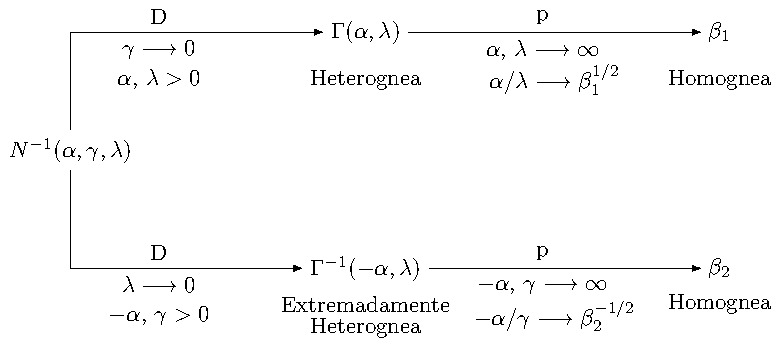
\includegraphics[scale=1]{../../Figures/Tesis/Capitulo4/RelacionInversaGaussiana.pdf}
	\caption{\label{RelacionInversaGaussiana}Comportamiento asintótico da la distribución $N^{-1}(\alpha,\gamma,\lambda)$.} %Fuente Canada Centre for Remote Sensing \citet{ccrs2001}.}
\end{figure} 

Este comportamiento asintótico muestra que tanto retrodispersores homogéneos como heterogéneos y extremadamente heterogéneos pueden tratarse a partir de la distribución $N^{-1}(\alpha,\gamma,\lambda)$.
%Cabe señalar que, por la forma en que fué definido el número de looks $L$ debería, en principio, ser un número entero. En general este parámetro se lo considera conocido porque viene con la información de la imagen. En el caso que no sea conocido se estima a partir de los datos reales debido, entre otros
%razones, el hecho de que la media de intensidad se toma sobre observaciones correlacionadas.
%Por lo tanto, n es, en general, llamado número equivalente de miradas. Para valores altos
%de n la distribución r (n, n) se acerca a la distribución gaussiana, que puede ser
%explicado por el Teorema del límite central


\section{Modelo para el Retorno}
\label{Retorno}

De acuerdo a lo visto en las secciones~\ref{ModeloSpeckle} y~\ref{ModeloBackscatter} surge un modelo para la intensidad del retorno para datos multilook a partir del modelo multiplicativo definido en la sección~\ref{ModeloMultiplicativo}.
\begin{equation*}
Z=X \cdot Y  
\end{equation*}
donde $X$ e $Y$ son variables aleatorias independientes que corresponden a la retrodispersión y al ruido speckle, respectivamente. 

 \citet{Frery99} proponen que $X \sim N^{-1}(\alpha,\lambda,\gamma )$, $Y \sim \Gamma(L,L)$, entonces $Z$ obedece una distribución $\mathcal G_I(\alpha,\lambda,\gamma,L )$, que es el modelo $\mathcal{G}$ para datos de intensidad. \citet{Frery97} presentan el modelo $\mathcal{G}$ para datos de amplitud a partir de un análisis similar.

Entonces, el retorno $Z \sim \mathcal{G}_I$ si su función de densidad está dada por
\begin{align}
\label{ModeloGI}
f_{\text{Z}}( z) =\frac{z^{L-1} L^L \sqrt{(\frac{\lambda}{\gamma})^{\alpha}}}{\Gamma(L)\text{K}_{\alpha}(2 \sqrt{\lambda \gamma})} \left(\dfrac{\gamma + Lz}{\lambda}\right)^{(\alpha-L)/2} \text{K}_{\alpha-L}(2\sqrt{\lambda(\gamma+Lz) })
\end{align}
donde $L\geq 1$ es el número de looks y el espacio paramétrico para $\alpha$, $\gamma$ y $\lambda$ es el mismo que en~\eqref{EspacioParametros}.

Cabe señalar que el número de looks $L$ debería ser, en principio, un número natural por la forma en que fué definido. En general este parámetro es considerado conocido porque viene con la información de la imagen, pero puede ser que no lo sea. En este caso se estima a partir de los datos de la imagen con muestras extraídas de zonas homogéneas y se llama número equivalente de looks (ENL). De acuerdo a \citet{anfinsen2009}, $\widehat{\text{ENL}}={1}/{\widehat{\text{CV}^2}(Z)}$ donde $\widehat{\text{CV}}(Z)={\widehat{\sigma}}/{\widehat\mu}$, con $\widehat{\sigma}$ es el desvío estandar muestral y $\widehat\mu$ la media muestral.

\citet{Frery99} obtienen casos particulares de la distribución $\mathcal{G}_I$ dependiendo del comportamiento asintótico de sus parámetros, esto se muestra en la figura~\ref{RelacionGI}.  
\begin{figure}[hbt]
	\centering    
	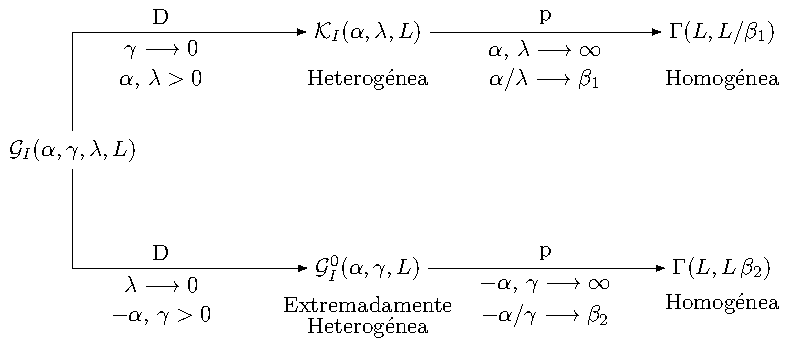
\includegraphics[scale=1]{../../Figures/Tesis/Capitulo4/RelacionGI.pdf}
	\caption{\label{RelacionGI}Comportamiento asintótico de la distribución $\mathcal{G}_I(\alpha,\gamma,\lambda,L)$.} %Fuente Canada Centre for Remote Sensing \citet{ccrs2001}.}
\end{figure} 

Se puede observar que, cuando 
\begin{itemize}
	\item $\gamma \longrightarrow 0$ y $\alpha,\lambda$ son positivos, $\mathcal{G}_I \stackrel{D}{\longrightarrow}\mathcal{K}(\alpha,\lambda,L)$.
	\item $\lambda \longrightarrow 0$ y $-\alpha,\gamma$ son positivos, $\mathcal{G}_I\stackrel{D}{\longrightarrow}\mathcal{G}_I^0(\alpha,\gamma,L)$.
\end{itemize}

Entonces, bajo el modelo multiplicativo, tenemos los siguientes modelos para el retorno que son casos particulares de la distribución $\mathcal{G}_I$. Si el ruido speckle $Y \sim \Gamma(L,L)$ y considerando diferentes modelos para $X$, tenemos las siguientes distribuciones para la intensidad del retorno $Z$.
\begin{itemize}
	\item Si $X \sim \Gamma(\alpha,\lambda)$, entonces $Z \sim \mathcal{K}(\alpha,\lambda,L)$ con $\gamma, \, \lambda >0$ y $L \geq 1$.
	\item Si $X \sim \Gamma^{-1}(-\alpha,\gamma)$, entonces $Z \sim \mathcal{G}_I^0(\alpha,\gamma,L)$ con $-\alpha, \, \gamma >0$ y $L \geq 1$.
\end{itemize}

Por otro lado y de acuerdo a la parametrización de la distribución Gaussiana Inversa dada en~\eqref{OtraIG}, si $X\sim IG(\omega,\eta)$ e $Y \sim \Gamma(L,L)$ el retorno $Z$ queda modelado por la distribución $ \mathcal{G}^H(\omega,\eta,L)$ con $\omega, \, \eta >0$ y $L \geq 1$, donde la función de densidad está dada por 
\begin{align}
\label{ModeloGH}
f_{\text{Z}}( z) =\frac{L^L \sqrt{\frac{2 \omega  \eta }{\pi }} e^{\omega } \left(\frac{\omega }{\eta  (\omega  \eta +2 L
		x)}\right)^{\frac{L}{2}+\frac{1}{4}} x^{L-1} K_{-\left(L+\frac{1}{2}\right)}\left(\sqrt{\frac{\omega 
			(\omega  \eta +2 L x)}{\eta }}\right)}{\Gamma (L)}
\end{align}
Esta familia de distribuciones $\mathcal{G}^H(\gamma,\lambda,L)$ para el retorno fueron aplicadas a datos SAR en \citet{Buemi2009} y \citet{Jacobo2005}.

%La familia de distribuciones $\mathcal{G}_I$ modelan mejor datos que provienen de áreas heterogéneas y extremadamente heterogéneas que la familia $\mathcal{K}$ \citet{Frery97,MejailJacoboFreryBustos:IJRS}. Mejail et al. \citet{MejailJacoboFreryBustos:IJRS} mostraron que, con una elección adecuada de los parámetros,
%la distribución $\mathcal{G}_I$ puede aproximar muy bien a la distribución  $\mathcal{K}$. Por estas razones, el modelo $\mathcal{G}_I$ se llama Modelo Universal para datos SAR \citet{FreryLibro2019} y es el modelo utilizado en esta tesis.

\section{Modelo $\mathcal{G}_I^0$}
\label{ModeloGI0}

Diremos que si $Z=X \cdot Y$ con $X \sim \Gamma^{-1}(-\alpha,\gamma)$ e $Y \sim \Gamma(L,L)$ independiente, el retorno $Z \sim \mathcal{G}_I^0(\alpha,\gamma,L)$. Su función de densidad está dada por 
\begin{equation}
f_{\mathcal{G}_I^{0}}( z) =\frac{L^{L}\Gamma ( L-\alpha
	) }{\gamma ^{\alpha }\Gamma ( -\alpha ) \Gamma (
	L) }\cdot  
\frac{z^{L-1}}{( \gamma +zL) ^{L-\alpha }},%
\label{ec_dens_gI0}
\end{equation}
donde $-\alpha,\gamma ,z>0$ y $L\geq 1$.

De acuerdo a \citet{gambini2015} los momentos de orden $r$ están dados por
\begin{equation}
E(Z^r) =\Big(\frac{\gamma}{L}\Big)^r\frac{\Gamma ( -\alpha-r )}{ \Gamma (-\alpha) }
\frac{\Gamma (L+r )}{\Gamma (L)},
\label{moments_gI0}
\end{equation}
y son finitos si $\alpha<-r$. Por lo tanto para que la $E(Z)$ sea finita el parámetro $\alpha<-1$. Este punto hay que tenerlo en cuenta al momento de la estimación del parámetro $\alpha$.

En la figura~\ref{DensidadGI0L03} se muestra el gráfico de la densidad $\mathcal{G}_I^0$ para $L=3$ y tres diferentes valores de $\alpha$, en escala lineal~\ref{EscalaLineal} y en escala semilogarítmica~\ref{EscalaSemiLog}. Se puede observar en~\ref{EscalaSemiLog} la diferencia que existe en el comportamiento de las colas de la distribución, estudiaremos este comportamiento en la subsección~\ref{colas}. Se puede observar que cuanto mayor es el parámetro de textura más pesadas son las colas de la distribución.

\begin{figure}[hbt]
	\centering    
	\subfigure[Escala lineal\label{EscalaLineal}]{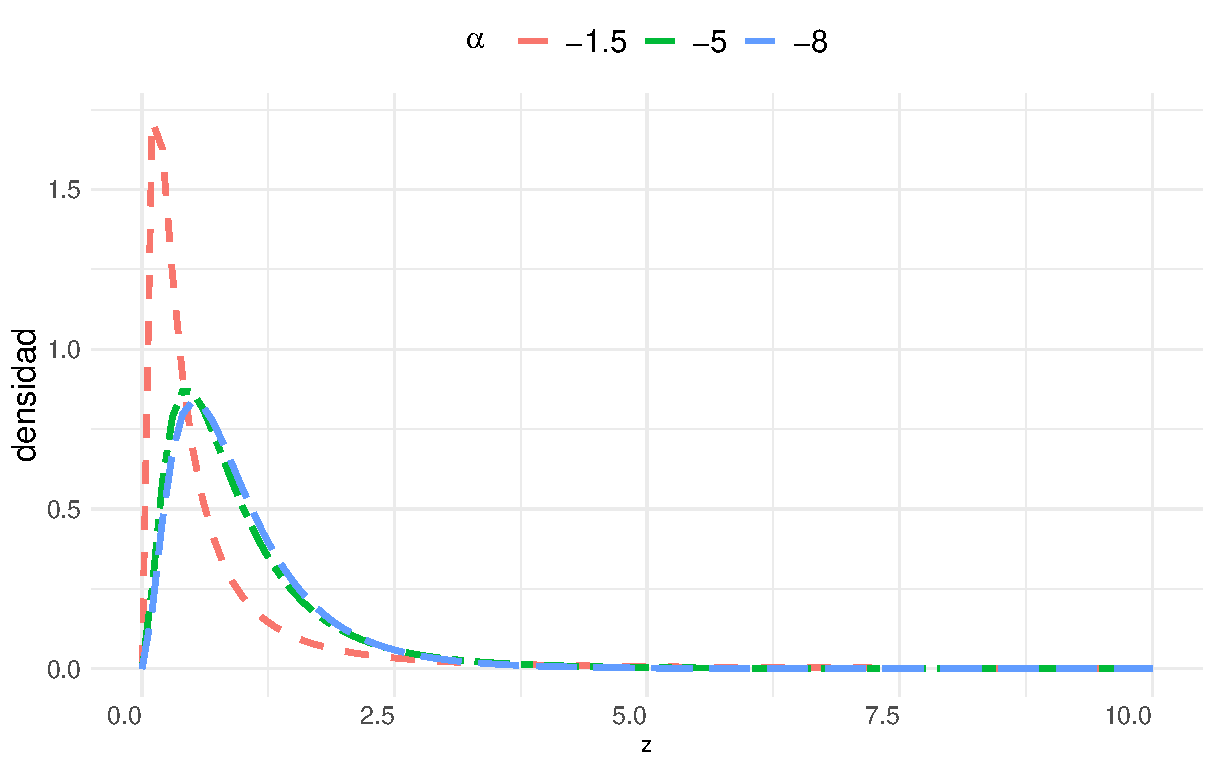
\includegraphics[width=.48\linewidth]{../../Figures/Tesis/Capitulo4/DensidadGI0L3.pdf}}
	\subfigure[Escala semilogarítmica\label{EscalaSemiLog}]{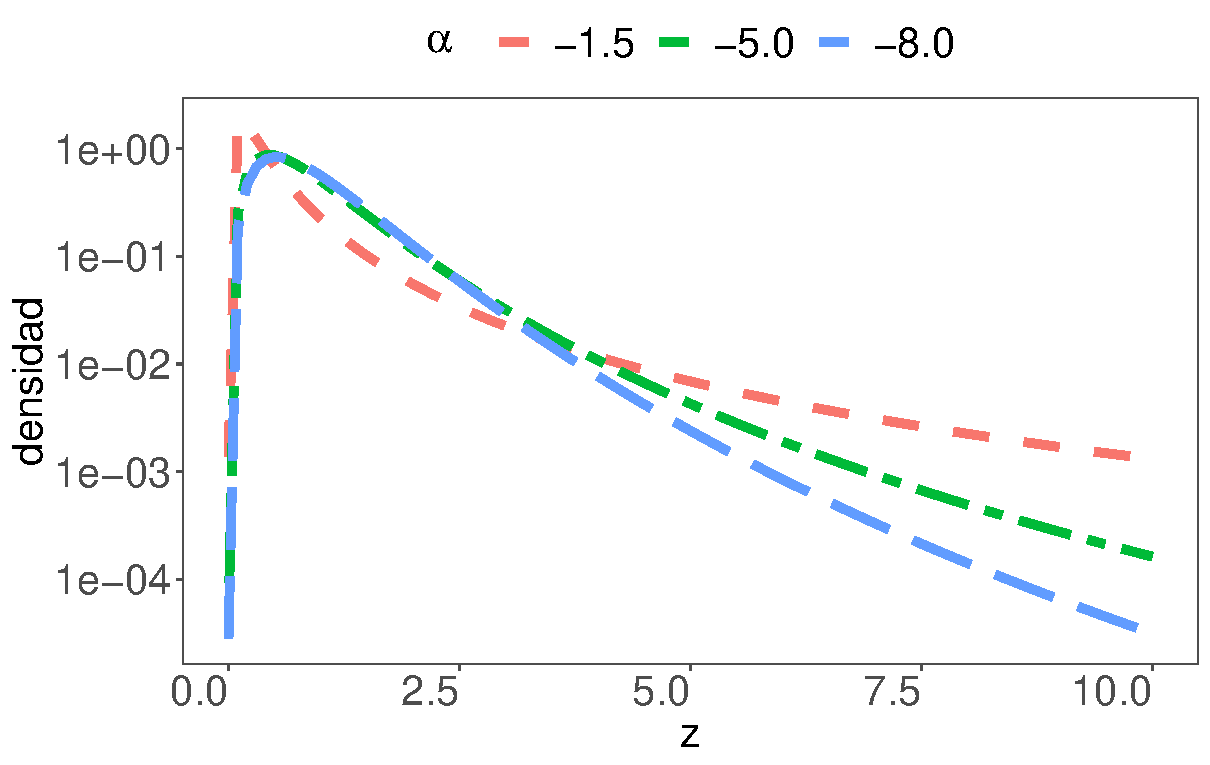
\includegraphics[width=.48\linewidth]{../../Figures/Tesis/Capitulo4/DensGI0_L3_Semilog.pdf}}
	\caption{\label{DensidadGI0L03}Densidad $\mathcal{G}_I^0$ para $L=3$ y $\alpha=-1.5, \, -5, \, -8$.}
\end{figure} 

En la figura~\ref{DensidadGI0TodoL} se muestra el gráfico de la densidad $\mathcal{G}_I^0$ para $L=1, \, 3, \, 8$ y $\alpha= -5$. Se puede obervar el efecto multilook, a medida que el número de looks aumenta, las colas son menos pesadas.

\begin{figure}[hbt]
	\centering    
	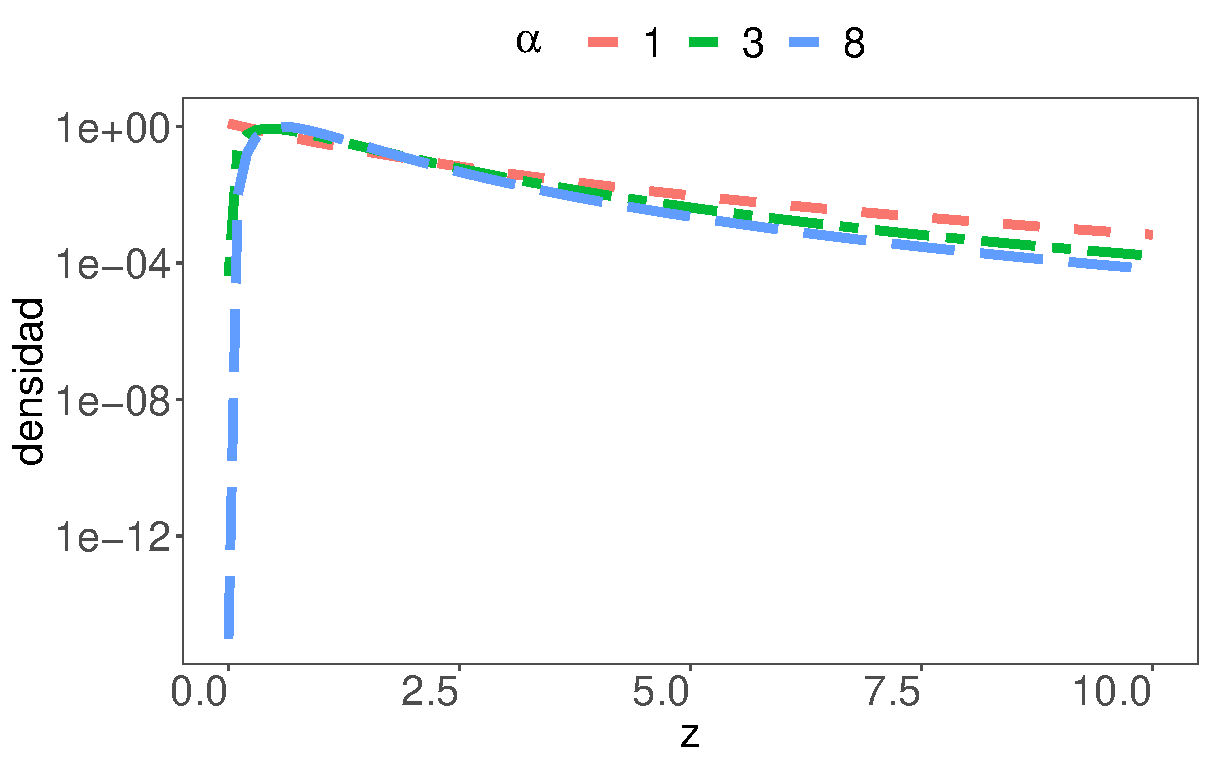
\includegraphics[width=.5\linewidth]{../../Figures/Tesis/Capitulo4/DensGI0_TodoL_Semilog.pdf}
	\caption{\label{DensidadGI0TodoL}Densidad $\mathcal{G}_I^0$ para $L=1, \, 3, \, 8$ y $\alpha= -5$.}
\end{figure} 

Bajo este modelo se pueden caracterizar regiones con diferentes grado de textura a través de los parámetros de la distribución $\mathcal{G}_I^{0}$. Para valores de $\alpha$ cercanos a cero (típicamente en el intervalo $(-3,0)$), la zona de la imagen corresponde a una región muy texturada, como es el caso de las zonas urbanas en las imágenes SAR. A medida que el valor del parámetro $\alpha$ disminuye, corresponde a zonas con cada vez menos textura, como son las regiones de forestación (usualmente $(-6,-3]$) y pastura (en $(-\infty,-6)$). Por otro lado, el parámetro $\gamma$ (llamado parámetro de escala) posee una interpretación en términos del brillo. Cuanto mayor es su valor, mayor intensidad posee la imagen en esa región. Por estas razones, la estimación precisa de los parámetros es de suma importancia en el análisis de imágenes con ruido speckle. 



%%%%%%%%%%%%%%%%%%%%%%%%%%%%%%%%%%%%%%%%%%%%%%%%%%%%%%%%%%%%
\section{Resultados Teóricos}
\label{ResultadosTeoricosGI0}

En esta sección se darán nuevos resultados teóricos presentados en \citet{gambini2015}, que muestran que la distribución $\mathcal{G}_I^0$ es una distribución de colas pesadas. Esto explica en parte los problemas que se enfrentan al buscar estimadores de los parámetros de esta distribución.  También se presentan nuevos resultados sobre el comportamiento asintótico de la distribución $\mathcal{G}_I^0$ respectos de sus parámetros, que se necesitarán para demostrar la consistencia del estimador del parámetro de textura $\alpha$ propuesto en esta tesis.

\subsection{$\mathcal{G}_I^0$ distribución de colas pesadas}
\label{colas}
Siguiendo a \citet{Gre,Jorgensen,Rojo} daremos las siguientes definiciones.

\begin{definition} \label{Def:lenta}
	La función $\ell\colon\mathbb R \to\mathbb R$ es de variación lenta en el infinito si para todo $t>0$ vale que
	$$
	\lim_{x\to+\infty}\dfrac{\ell (tx)}{\ell(x)}=1.
	$$
\end{definition}

\begin{definition} 
	Una función de densidad de probabilidad $f(x)$ tiene colas pesadas si para algún $\eta >0$ vale que
	$$
	f(x)=\ell(x)  x^{-\eta},
	$$
	donde $\ell$ es una función de variación lenta en el infinito y $\eta$ es el índice de la cola.
\end{definition}
Cuanto menor es el índice de la cola, más propensa es la distribución a producir observaciones extremas.

\begin{proposition}
	La distribución $\mathcal G_{I}^0$ tiene colas pesadas con índice de la cola igual a $1-\alpha$.
\end{proposition}
\begin{proof}
	Si definimos $\ell(x)=f_{\mathcal G_I^0}(x) x^{-\alpha+1}$ tenemos que
	\begin{align*}
	\lim_{x\to+\infty}\frac{\ell(t x)}{\ell(x)}&=\lim_{x\to+\infty}\frac{(tx)^{L-1} \, (Ltx+\gamma)^{\alpha-L} \, (tx)^{1-\alpha}}{x^{L-1} \, (Lx+\gamma)^{\alpha-L} \, x^{1-\alpha}}\\
	&=\lim_{x\to+\infty}t^{L-\alpha}\left(\frac{Lx+\gamma}{L tx+\gamma}\right)^{L-\alpha}=1.
	\end{align*}
	Esto vale para todo $t>0$, por lo tanto $\ell$ es de variación lenta en el infinito.
\end{proof}
Se puede ver que el índice de la cola es una función decreciente de $\alpha$, entonces la distribución $\mathcal G_I^0$ es más propensa a producir valores extremos cuando el parámetro de textura es más grande. Esto va de acuerdo a lo mostrado en la figura~\ref{DensidadGI0L03}.

\subsection{Comportamiento asintótico de la distribución $\mathcal{G}_I^0$.}
Estos resultados se probarán considerando el caso $E(Z)=1$ que nos da una relación entre los parámetros de la distribución $\mathcal{G}_I^0$: $\gamma^*=-\alpha-1$. Como el parámetro $\gamma$ es considerado un parámetro de escala, con esta relación logramos que los resultados para diferentes áreas resulten comparables.
 
En este caso se puede escribir a $f_{\mathcal{G}_I^0}\pa{z}$ en términos de $\gamma$. De esta forma, la función de distribución del modelo $\mathcal{G}_I^0$ bajo esta condición queda:
\begin{align}
\label{fenfunciondegamma}
f_{\gamma}\pa{z}=\frac{\Gamma\pa{L+\gamma+1}}{\Gamma\pa{\gamma+1}\Gamma\pa{L}}
\pa{\frac{L}{\gamma}}^L \frac{z^{L-1}}{\pa{1+\frac{Lz}{\gamma}}^{L+\gamma+1}}.
%f_{\mathcal{G}_I^0}\pa{z} = \frac{\Gamma\pa{L+\gamma+1}}{\Gamma\pa{\gamma+1}\Gamma\pa{L}}
%L^{-1-\gamma} z^{-2-\gamma} \gamma^{\gamma +1} \pa{1+\frac{\gamma}{L z}}^{-\gamma -L-1}.
\end{align}

Vamos a utilizar esta forma de escribir a $f_{\mathcal{G}_I^0}\pa{z}$ en las proposiciones~\ref{conv1} y ~\ref{conv2}.

\begin{proposition}
	\label{conv1}
	Para todo intervalo compacto $[z_{1},z_{2}]\subset\pa{0,\infty}$, $f_{\mathcal{G}_I^0}\pa{z}$ converge
	uniformemente a $\Gamma(\text{L,L})$ en $[z_{1},z_{2}]$ si $\alpha\to -\infty$,
	donde $\Gamma(\text{L,L})$ es la función de densidad del modelo $\Gamma$ con parámetros $\pa{\text{L,L}}$.
\end{proposition}

\begin{dem}
Si consideramos $f_{\mathcal{G}_I^0}\pa{z}$ escrita como en~\eqref{fenfunciondegamma} estudiar la convergencia de $f_{\mathcal{G}_I^0}\pa{z}$ cuando $\alpha\to -\infty$ es equivalente a estudiar el $\lim\limits_{\gamma\to+\infty} f_{\gamma}\pa{z}$. 
		
Si llamamos:
	\begin{align*}
		a\pa{\gamma} &= \frac{\Gamma\pa{\gamma+1}\e^{\gamma}}{\sqrt{2\pi}\gamma^{\gamma+1/2}},\\
%		b\pa{L,\gamma,z} &=L\gamma^{L-1}\pa{\frac{\frac{Lz}{\gamma}}{1+\frac{Lz}{\gamma}}}^{L-1} \text{ y }\\
%		c\pa{L,\gamma,z} &= \pa{1+\frac{Lz}{\gamma}}^{-2-\gamma},
	\end{align*}
entonces 
\begin{align}
\label{GIOfunciongamma}
f_{\gamma}\pa{z} = \frac{a\pa{L+\gamma}}{a\pa{\gamma}\Gamma\pa{L}}\e^{-L}\pa{1+\frac{L}{\gamma}}^{L+\gamma+1/2} \dfrac{L^L z^{L-1}}{\left(1+\dfrac{L z}{\gamma}\right)^{L+\gamma +1}}.
\end{align}

%\begin{align*}
%	\lim_{\gamma\to+\infty}\frac{\Gamma\pa{L+\gamma+1}}{\Gamma\pa{\gamma+1}\Gamma\pa{L}}
%	\frac{L}{\gamma}\pa{\frac{\frac{Lz}{\gamma}}{1+\frac{Lz}{\gamma}}}^{L-1}
%	\pa{1+\frac{Lz}{\gamma}}^{-2-\gamma},
%\end{align*}

De la fórmula de Stirling se obtiene
	\begin{align*}
	% \lim_{\gamma\to+\infty} a\pa{L,\gamma} = 
	% \al \lim_{\gamma\to+\infty}\frac{\Gamma\pa{L+\gamma+1}\e^{L+\gamma}}{\sqrt{2\pi}\pa{L+\gamma}^{L+\gamma+1/2}} = 1,\\
	\lim_{\gamma\to+\infty} a\pa{\gamma} = 
	\al \lim_{\gamma\to+\infty}\frac{\Gamma\pa{\gamma+1}\e^{\gamma}}{\sqrt{2\pi}\gamma^{\gamma+1/2}} = 1,
	\end{align*}
	
entonces
	\begin{align*}
	1=\lim_{\gamma\to+\infty} \frac{a\pa{L+\gamma}}{a\pa{\gamma}} = 
	\al \lim_{\gamma\to+\infty}\frac{\Gamma\pa{L+\gamma+1}}{\Gamma\pa{\gamma+1}}
	\e^{L}\gamma^{-L}\pa{1+\frac{L}{\gamma}}^{-L-\gamma-1/2}.
	\end{align*}

	Por otro lado, se verifica 
	\begin{align}
	\label{b}
	\lim_{\gamma\to+\infty} \left(1+\dfrac{L}{\gamma}\right)^{L+\gamma +1/2}=e^L,\\
	\label{c}
	\lim_{\gamma\to+\infty} \left(1+\dfrac{L z}{\gamma}\right)^{-(L+\gamma +1)}=e^{-L z}
%	\label{b}
%	\nonumber \lim_{\gamma\to+\infty} b\pa{L,\gamma,z} =
%	\al \lim_{\gamma\to+\infty}L\gamma^{L-1}\pa{\frac{\frac{Lz}{\gamma}}{1+\frac{Lz}{\gamma}}}^{L-1} \\
%	= \al \lim_{\gamma\to+\infty} \frac{L^{L} z^{L-1}}{\pa{1+\frac{Lz}{\gamma}}^{L-1}} = L^{L} z^{L-1},\\
%	\lim_{\gamma\to+\infty} c\pa{L,\gamma,z} = \al \lim_{\gamma\to+\infty}\pa{1+\frac{Lz}{\gamma}}^{-2-\gamma} = \e^{-Lz},
%	\label{c}
	\end{align}
	donde la convergencia en~\eqref{c} es uniforme en $[z_{1},z_{2}]$.
	
	Entonces se obtiene que $\lim\limits_{\gamma\to+\infty}f_{\gamma}\pa{z} = L^{L}/\Gamma\pa{L}\,\e^{-Lz}z^{L-1}$ uniformemente en $[z_{1},z_{2}]$, donde $f_{\gamma}\pa{z}$ es la función de densidad dada en~\eqref{GIOfunciongamma}.
\end{dem}

La figura~\ref{ConvInfinito} muestra la convergencia uniforme de $f_{\mathcal{G}_I^0}\pa{z}$ a $\Gamma(3,3)$, cuando $\alpha \to -\infty$ y $L=3$. 
El área gris es una banda de ancho $\epsilon=0.1$ alrededor de la función de densidad $\Gamma(3,3)$ (línea sólida). 
La línea punteada y la línea discontinua representan $f_{\mathcal{G}_I^0}\pa{z}$ para $\alpha=-20$ y $\alpha=-8$ respectivamente. 
Se puede ver que, cuando $\alpha$ disminuye, $f_{\mathcal{G}_I^0}\pa{z}$ cae dentro del área gris. 
Mas aún, para este valor de $\epsilon$, $f_{\mathcal{G}_I^0}(-20)$ ya cae dentro de esa banda.


\begin{figure}[hbt]
\begin{center}
	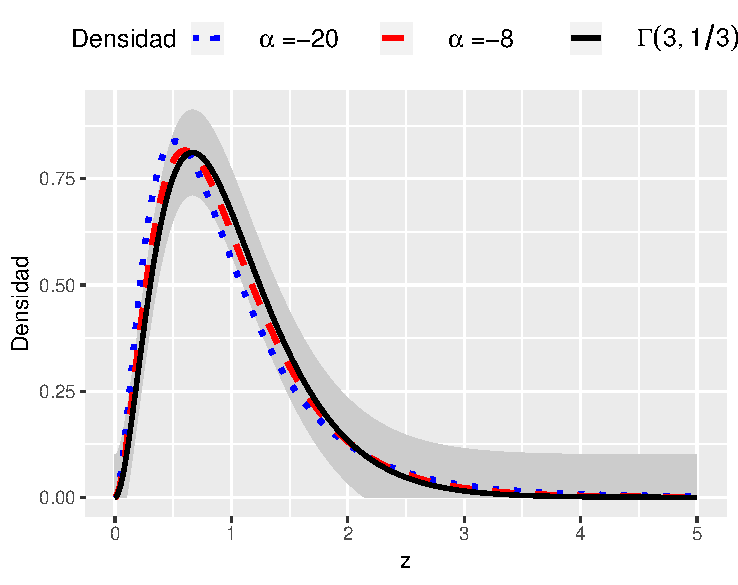
\includegraphics[scale=0.8]{../../Figures/Tesis/Capitulo4/ConvUniformeMenosInfinito2.pdf}
	\caption{\label{ConvInfinito}\small{Convergencia uniforme de $f_{\mathcal{G}_I^0}\pa{z}$ a $\Gamma(3,3)$ cuando $\gamma=\gamma^*$, $\alpha \to -\infty$, $L=3$ y $\epsilon=0.1$.}}
\end{center}
\end{figure} 


\begin{proposition}
	\label{conv2}
	Para todo intervalo compacto $[z_{1},z_{2}]\subset\pa{0,\infty}$, $f_{\mathcal{G}_I^0}\pa{z}$ converge
	uniformemente a $0$ en $[z_{1},z_{2}]$, si $\alpha\to -1^{-}$.
\end{proposition}
\begin{dem}
	En forma equivalente a la proposición~\ref{conv1} y usando la relación entre $\alpha$ y $\gamma$, estudiar la convergencia de $f_{\mathcal{G}_I^0}\pa{z}$ cuando $\alpha\to -1^{-}$ es equivalente a estudiar ese límite cuando ${\gamma\to 0^{+}}$.
	De~\eqref{fenfunciondegamma}:
	\begin{align*}
	f_{\gamma}\pa{z} = &\frac{\Gamma\pa{L+\gamma+1}}{\Gamma\pa{\gamma+1}\Gamma\pa{L}}
	L^{L} \frac{z^{L-1}}{(\gamma+Lz)^{L+\gamma+1}} \gamma^{\gamma +1}  \\
	\leq& \frac{\Gamma\pa{L+\gamma+1}}{\Gamma\pa{\gamma+1}\Gamma\pa{L}}
	L^{L} \frac{z_2^{L-1}}{(\gamma+Lz_1)^{L+\gamma+1}} \gamma^{\gamma +1} 
	\end{align*}
	Dado que $\Gamma$ es una función continua, para $z \in [z_{1},z_{2}]$, $\lim\limits_{\gamma\to0^+} f_{\gamma}\pa{z}=0$ uniformemente en $z$, con lo que se obtiene el resultado.
\end{dem}

La figura~\ref{ConvEnCero} muestra la convergencia uniforme de $f_{\mathcal{G}_I^0}\pa{z}$ cuando $\alpha \to -1$ y $L=3$. La banda gris es de ancho $\epsilon=0.2$ alrededor del eje $z$. 
Se graficaron tres diferentes densidades con líneas punteada, discontinua y sólida, las cuales representan $f_{\mathcal{G}_I^0}\pa{z}$ para $\alpha=-1.01, \ -1.2$ y $-1.5$ respectivamente. 
Se puede ver que cuando el valor de $\alpha$ se acerca a $-1$, $f_{\mathcal{G}_I^0}\pa{z}$ se aplana a $0$, excepto para $z=0$. 
Para  $\epsilon=0.2$ y cualquier intervalo $[z_1,z_2]$ considerado, $f_{\mathcal{G}_I^0}\pa{z}$ cae dentro de esta banda para $\alpha$ suficientemente cercano a $-1$. 
Por ejemplo, para el intervalo $[1.5,2]$ y para este valor de $\epsilon$, $f_{\mathcal{G}_I^0}\pa{z}$ entra en la banda gris desde $\alpha=-1.5$. 
Si el intervalo es $[0.5,1]$ esto sucede a partir de $\alpha=-1.01$.



\begin{figure}[hbt]
	\centering    
	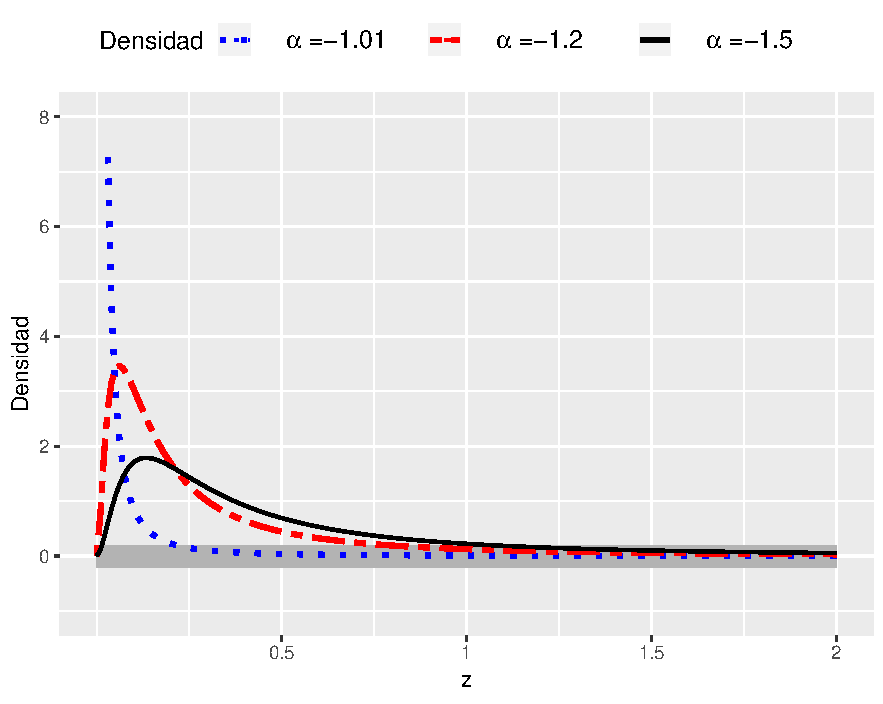
\includegraphics[width=0.8\linewidth]{../../Figures/Tesis/Capitulo4/ConvUnifEnCero.pdf}
	\caption{\label{ConvEnCero}Convergencia uniforme de $f_{\mathcal{G}_I^0}\pa{z}$ a $0$ cuando $\gamma=\gamma^*$, $\alpha \to -1$, $L=3$ y $\epsilon=0.2$.}
\end{figure}

\section{Conclusiones}

En este capítulo presentamos varias distribuciones que se utilizan para modelar datos provenientes de imágenes SAR:
\begin{itemize}
	\item Los llamados modelos empíricos que son distribuciones que se propopnen para ajustar datos SAR, como la distribución Lognormal, Weibull entre otras.
	\item El modelo multiplicativo, que establece que el retorno $Z$ se modela como el producto de dos variables aleatorias: $X$ para la retrodispersión e $Y$ para el ruido speckle.
\end{itemize} 

Mostramos un abordaje donde se explica la naturaleza multiplicativa del ruido speckle. A partir de esto se propuso modelar al ruido speckle $Y$ con una distribución $\Gamma(L,L)$ en el caso de datos en formato intensidad y monopolarizados, donde $L$ es el número de looks. En cuanto a la retrodispersión $X$ se propone modelarla con una distribución Gaussiana Inversa Generalizada $N^{-1}(\alpha,\gamma,\lambda)$. Para valores particulares de los parámetros de la distribución $N^{-1}(\alpha,\gamma,\lambda)$, se obtienen las distribuciones $\Gamma(\alpha,\lambda)$, $\Gamma^{-1}(\alpha,\gamma)$ e $IG(\gamma, \lambda)$. Bajo el modelo multiplicativo estas distribuciones para la retrodispersión dan origen a las distribuciones $\mathcal{K}$, $\mathcal{G}_I^0$ y $\mathcal{G}^H$ para el retorno $Z$, respectivamente. 

En esta tesis utilizamos el modelo $\mathcal{G}_I^0$ para datos de intensidad. Presentamos la función de distribución y demostramos que es una distribución que tiene colas pesadas.

Asimismo demostramos resultado sobre la convergencia uniforme de la distribución $\mathcal{G}_I^0$ cuando el parámetro de textura se acerca a $-1$ y a $-\infty$ para el caso donde $E(Z)=1$.




%\begin{proposition}
%	\label{pr: falpha>0}
%	Para todo $\alpha\in I$, existe $U$ un entorno compacto de $\alpha$ tal que
%	$\inf\limits_{\alpha'\in I-U}d_{T}\pa{f_{\alpha'};f_{\alpha}}>0$.
%\end{proposition}
%\begin{dem}
%	Siendo que $f_{\alpha}\ne f_{\Gamma,L,L}$, existe $[z_{1},z_{2}]\subset\pa{0,\infty}$, tal que
%	\begin{align*}
%	\int_{z_{1}}^{z_{2}}\frac{\pa{f_{\alpha}\pa{z}-f_{\Gamma,L,L}\pa{z}}^{2}}
%	{f_{\alpha}\pa{z}+f_{\Gamma,L,L}\pa{z}}dz >0,
%	\end{align*}
%	entonces
%	\begin{align*}
%	\liminf_{\alpha'\to-\infty} d_{T}\pa{f_{\alpha'};f_{\alpha}} 
%	\ge \al \liminf_{\alpha'\to-\infty}\int_{z_{1}}^{z_{2}}\frac{\pa{f_{\alpha}\pa{z}-f_{\alpha'}\pa{z}}^{2}}
%	{f_{\alpha}\pa{z}+f_{\alpha'}\pa{z}}dz \\
%	= \al \int_{z_{1}}^{z_{2}}\frac{\pa{f_{\alpha}\pa{z}-f_{\Gamma,L,L}\pa{z}}^{2}}
%	{f_{\alpha}\pa{z}+f_{\Gamma,L,L}\pa{z}}dz >0.
%	\end{align*}
%	De la misma forma
%	\begin{align*}
%	\liminf_{\alpha'\to-1^{-}} d_{T}\pa{f_{\alpha'};f_{\alpha}} 
%	\ge \al \liminf_{\alpha'\to-1^{-}}\int_{z_{1}}^{z_{2}}\frac{\pa{f_{\alpha}\pa{z}-f_{\alpha'}\pa{z}}^{2}}
%	{f_{\alpha}\pa{z}+f_{\alpha'}\pa{z}}dz \\
%	= \al \int_{z_{1}}^{z_{2}}f_{\alpha}\pa{z}dz >0,
%	\end{align*}
%	lo que prueba la proposición.
%\end{dem}
%\begin{corollary}
%	Si $\set{\alpha_{k}}_{k\in\N}$ una sucesión de $I$ tal que $d_{T}\pa{f_{\alpha_{k}};f_{\alpha}}\to 0$,
%	entonces $\alpha_{k}\to\alpha$.
%\end{corollary}
%\begin{dem}
%	Es consecuencia de las proposiciones \ref{pr: convergencia} y \ref{pr: falpha>0}.
%\end{dem}

